\documentclass{article}\usepackage[]{graphicx}\usepackage[]{color}
%% maxwidth is the original width if it is less than linewidth
%% otherwise use linewidth (to make sure the graphics do not exceed the margin)
\makeatletter
\def\maxwidth{ %
  \ifdim\Gin@nat@width>\linewidth
    \linewidth
  \else
    \Gin@nat@width
  \fi
}
\makeatother

\definecolor{fgcolor}{rgb}{0.345, 0.345, 0.345}
\newcommand{\hlnum}[1]{\textcolor[rgb]{0.686,0.059,0.569}{#1}}%
\newcommand{\hlstr}[1]{\textcolor[rgb]{0.192,0.494,0.8}{#1}}%
\newcommand{\hlcom}[1]{\textcolor[rgb]{0.678,0.584,0.686}{\textit{#1}}}%
\newcommand{\hlopt}[1]{\textcolor[rgb]{0,0,0}{#1}}%
\newcommand{\hlstd}[1]{\textcolor[rgb]{0.345,0.345,0.345}{#1}}%
\newcommand{\hlkwa}[1]{\textcolor[rgb]{0.161,0.373,0.58}{\textbf{#1}}}%
\newcommand{\hlkwb}[1]{\textcolor[rgb]{0.69,0.353,0.396}{#1}}%
\newcommand{\hlkwc}[1]{\textcolor[rgb]{0.333,0.667,0.333}{#1}}%
\newcommand{\hlkwd}[1]{\textcolor[rgb]{0.737,0.353,0.396}{\textbf{#1}}}%

\usepackage{framed}
\makeatletter
\newenvironment{kframe}{%
 \def\at@end@of@kframe{}%
 \ifinner\ifhmode%
  \def\at@end@of@kframe{\end{minipage}}%
  \begin{minipage}{\columnwidth}%
 \fi\fi%
 \def\FrameCommand##1{\hskip\@totalleftmargin \hskip-\fboxsep
 \colorbox{shadecolor}{##1}\hskip-\fboxsep
     % There is no \\@totalrightmargin, so:
     \hskip-\linewidth \hskip-\@totalleftmargin \hskip\columnwidth}%
 \MakeFramed {\advance\hsize-\width
   \@totalleftmargin\z@ \linewidth\hsize
   \@setminipage}}%
 {\par\unskip\endMakeFramed%
 \at@end@of@kframe}
\makeatother

\definecolor{shadecolor}{rgb}{.97, .97, .97}
\definecolor{messagecolor}{rgb}{0, 0, 0}
\definecolor{warningcolor}{rgb}{1, 0, 1}
\definecolor{errorcolor}{rgb}{1, 0, 0}
\newenvironment{knitrout}{}{} % an empty environment to be redefined in TeX

\usepackage{alltt}
\usepackage{catchfilebetweentags}

\usepackage[utf8]{inputenc}
%\usepackage[cp1251]{inputenc}
\usepackage[english]{babel}
\usepackage{indent first}
\usepackage[top=2 cm, bottom = 2 cm, left = 3 cm, right = 1.5 cm]{geometry}
\usepackage{amsmath}
\usepackage{amssymb}
\usepackage{amsthm}
\usepackage{graphicx}
\usepackage{wrapfig}
\usepackage{listings}
\usepackage{ mathrsfs }
\usepackage{subcaption}
\graphicspath{{images/}}
\renewcommand{\baselinestretch}{1.1}

\newtheorem*{theorem}{Theorem}
\IfFileExists{upquote.sty}{\usepackage{upquote}}{}
\begin{document}

\begin{center}
Federal State Autonomous Educational Institution
of High Professional Education
National Research University «Higher School of Economics»
\end{center}

\begin{center}
Faculty of Computer Science
School of Data Analysis and Artificial Intelligence
\end{center}

\vspace*{3 cm}

\begin{center} \huge
Report on the course \\ 
''Modern Methods of Data Analysis''.
\end{center}


\vspace*{1.5 cm}

\begin{center} \large
«Data Sciences» Master program \\
Lecturer: Boris G. Mirkin.
\end{center}


\begin{center} \large
\textbf{Authors:}\\
Cherny Artem \\
Ivanova Polina \\
Shvechikov Pavel \\
\end{center}
 
\newpage
\noindent \textbf{Dataset}: Online News Popularity Data Set. \\
URL: http://archive.ics.uci.edu/ml/datasets/Online+News+Popularity

\subsection*{Explanation of choice}
This dataset is based on recent articles, published in 2013--2015 years, so the data is actual up to now.   
Moreover, it is composed of different types of variables. 

\subsection*{Data Set Information}

\begin{itemize}
\item The articles were published by Mashable (www.mashable.com) and their content as the rights to reproduce it belongs to them. Hence, this dataset does not share the original content but some statistics associated with it. The original content could be publicly accessed and retrieved using the provided urls.  
\item Acquisition date: January 8, 2015  
\item The estimated relative performance values were estimated by the authors using a Random Forest classifier and a rolling windows as assessment method. See their article for more details on how the relative performance values were set.
\item From initial data-set we chose $34$ attributes and $10000$ instances (instances were chosen randomly).
\end{itemize}


\textbf{Attribute Information}:
\begin{enumerate}
\item \texttt{url}: URL of the article (non-predictive)
\item \texttt{timedelta}: Days between the article publication and the dataset acquisition (non-predictive) 
\item \texttt{n\_tokens\_title}: Number of words in the title 
\item \texttt{n\_tokens\_content}: Number of words in the content
\item \texttt{n\_unique\_tokens}: Rate of unique words in the content
\item \texttt{num\_hrefs}: Number of links 
\item \texttt{num\_self\_hrefs}: Number of links to other articles published by Mashable 
\item \texttt{num\_imgs}: Number of images  
\item \texttt{num\_videos}: Number of videos 
\item \texttt{average\_token\_length}: Average length of the words in the content
\item \texttt{num\_keywords}: Number of keywords in the metadata 
\item  \texttt{data\_channel\_is\_lifestyle}: Is data channel 'Lifestyle'? 
\item \texttt{data\_channel\_is\_entertainment}: Is data channel 'Entertainment'? 
\item \texttt{data\_channel\_is\_bus}: Is data channel 'Business'? 
\item \texttt{data\_channel\_is\_socmed}: Is data channel 'Social Media'? 
\item \texttt{data\_channel\_is\_tech}: Is data channel 'Tech'?  
\item \texttt{data\_channel\_is\_world}: Is data channel 'World'?

\item \texttt{self\_reference\_avg\_sharess}: Avg. shares of referenced articles in Mashable  
\item \texttt{weekday\_is\_monday}: Was the article published on a Monday?
\item \texttt{weekday\_is\_tuesday}: Was the article published on a Tuesday? 
\item \texttt{weekday\_is\_wednesday}: Was the article published on a Wednesday?
\item \texttt{weekday\_is\_thursday}: Was the article published on a Thursday? 
\item \texttt{weekday\_is\_friday}: Was the article published on a Friday?
\item \texttt{weekday\_is\_saturday}: Was the article published on a Saturday? 
\item \texttt{weekday\_is\_sunday}: Was the article published on a Sunday?
\item \texttt{global\_sentiment\_polarity}:     Text sentiment polarity
\item \texttt{global\_rate\_positive\_words}:    Rate of positive words in the content
\item \texttt{global\_rate\_negative\_words}:    Rate of negative words in the content
\item \texttt{rate\_positive\_words}:           Rate of positive words among non-neutral
\item \texttt{avg\_positive\_polarity}:         Avg. polarity of positive words
\item \texttt{avg\_negative\_polarity}:         Avg. polarity of negative  words 
\item \texttt{title\_sentiment\_polarity}:      Title polarity
\item \texttt{shares}:                        Number of shares (target)
\end{enumerate} 

\section{Assignment 1}
In the first task we consider the attribute called \texttt{shares},  which is the number of article shares in various social networks. Let construct a histogram and boxplot of chosen attribute (see Figure \ref{img:hist_boxplot_shares}). From the histogram wee can see, that the choosen attribute probably has a lognormal distribution, so we construct a new feautre \texttt{$\log$(shares)}. Histogram and boxplot for this new feature \texttt{$\log$(shares)} are presented on  Figure \ref{img:hist_boxplot_log_shares}. 


 
\begin{figure}[h!]
 \begin{center}
    \center 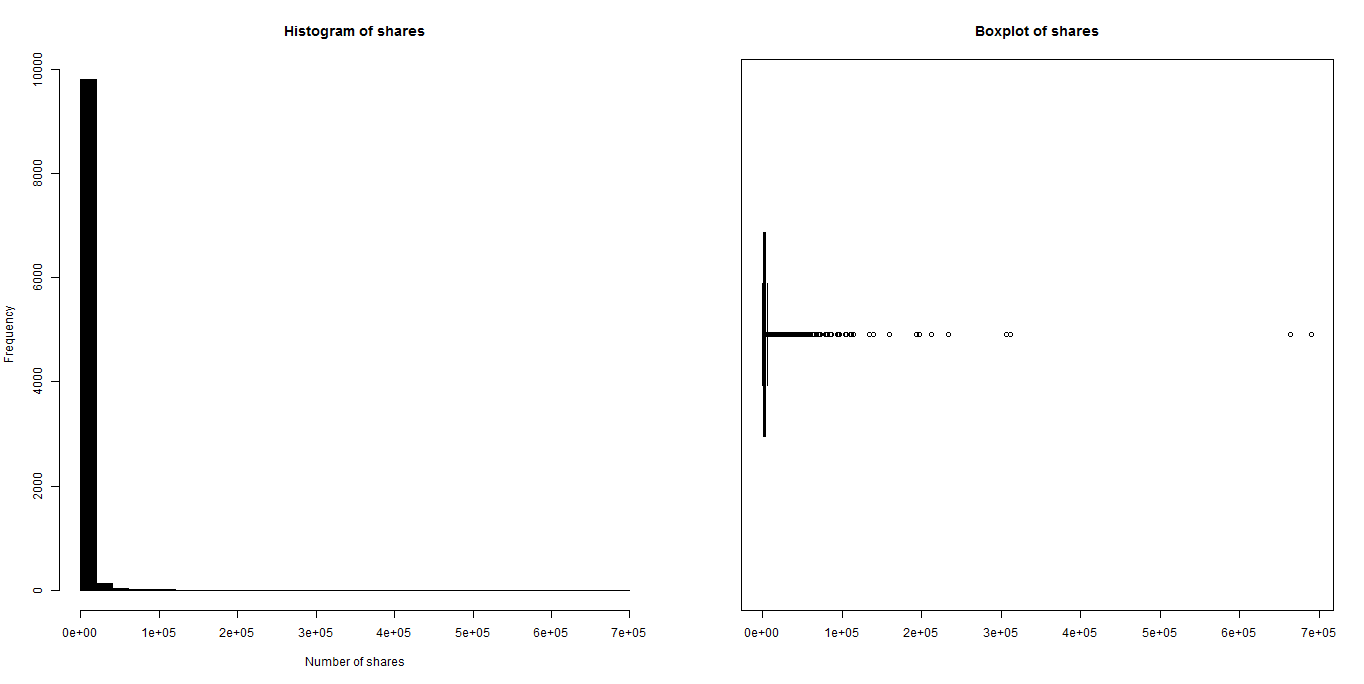
\includegraphics[width = 0.8\textwidth]{hist_boxplot_shares.png}
   \caption{}
   \label{img:hist_boxplot_shares}
 \end{center}
\end{figure} 
\begin{figure}[h!]
 \begin{center}
    \center 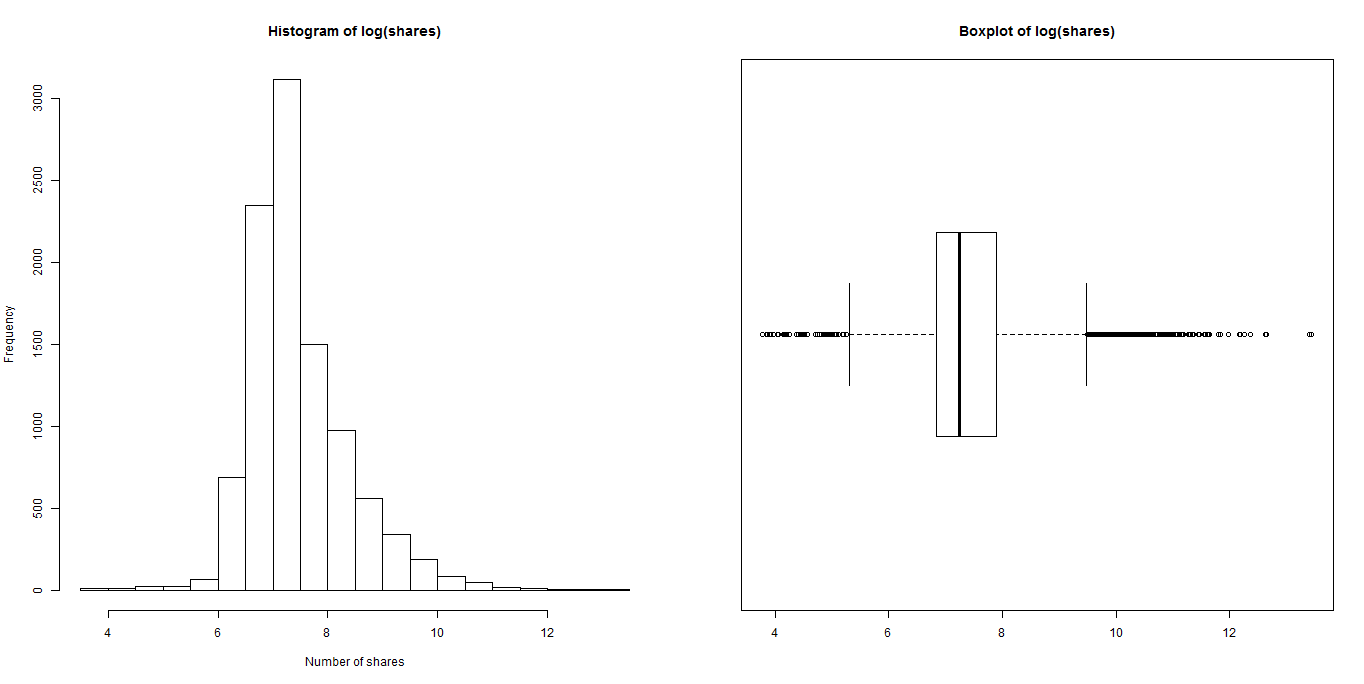
\includegraphics[width = 0.8\textwidth]{hist_boxplot_log_shares.png}
   \caption{}
   \label{img:hist_boxplot_log_shares}
 \end{center}
\end{figure}  

Below we will apply methods to the feature \texttt{$\log$(shares)} instead of \texttt{shares}. As we can see in the Table \ref{tbl:log_shares_stats1}, sample mean, median and mode of the \texttt{$\log$(shares)} agree closely with each other, indicating that distribution is similar to symmetric. If we look at the same characteristics for the \texttt{shares}, we can see that the mean is significantly greater than the median and the mode. That could be easily explained with the histogram of  \texttt{shares} (see Figure \ref{img:hist_boxplot_shares}), which shows that the majority of entities have less that $20\,000$, and very few have more than $600\,000$ shares.    


\begin{table}
\caption{Mean, median and mode for \texttt{shares} and \texttt{$\log$(shares)}} \label{tbl:log_shares_stats1}
\begin{center}
\begin{tabular}{|c|c|c|c|} 
 \hline
shares & Mean & Median & Mode \\ \hline
 & 3374.5 & 1400 & 1100 \\ \hline
$\log$(shares) & Mean & Median & Mode \\ \hline
 &  7.45 & 7.24 & 7.0 \\ \hline
\end{tabular}
\end{center}
\end{table}

\subsection*{Confidence intervals for the mean}
The task is to find three confidence intervals (CI) for the mean of \texttt{$\log$(shares)}. To do this, we make $N = 5000$ trials each of which consists of  sampling with replacement from initial set of \texttt{$\log$(shares)} and estimating the mean of population using that sampled data. The histogram of estimated means for the feature \texttt{$\log$(shares)} is presented on the Figure \ref{img:hist_means_of_log_shares}, and computed 95\% confidence intervals are shown in the Table 2 . The distribution of the means of \texttt{$\log$(shares)} is very similar to normal distribution, so pivotal and non-pivotal intervals are similar too. It is worth to mention that statistic confidence interval is much more wider compared with any of the others. 

\begin{figure}[h!]
 \begin{center}
    \center 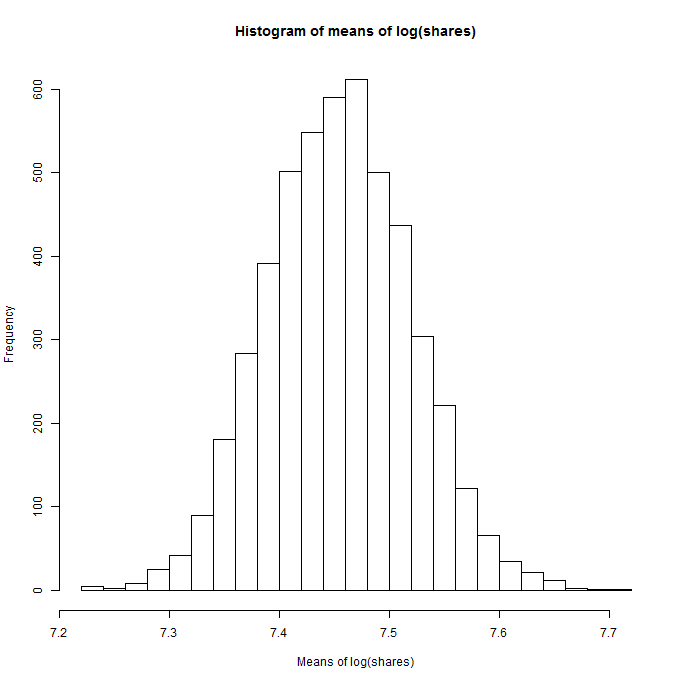
\includegraphics[width = 0.7\textwidth]{hist_means_of_log_shares.png}
   \caption{30-bin histogram of means of \texttt{$\log$(shares)}.}
   \label{img:hist_means_of_log_shares}
 \end{center}
\end{figure} 

\begin{table}
\caption{95\% confidence intervals (CI's) for mean of \texttt{$\log$(shares)}} \label{tbl:log_shares_stats}
\begin{center}
\begin{tabular}{|c|c|} 
 \hline
Mean & 7.45 \\ \hline 
Statistic CI & (5.94; 8.97) \\ \hline
Pivotal CI & (7.35; 7.56) \\ \hline
Nonpivotal CI & (7.33; 7.58) \\ \hline
\end{tabular}
\end{center}
\end{table}

\subsection*{Bootstraping the mode and the median}
The more the distribution resembles the  power law distribution, the more appropriate is to choose median of the distribution as the center value. That is because the median is very stable against outliers. 
And pivotal or non-pivotal bootstrap methods can be applied to medians. 

In case of mode it is hard to decide when the  bootstrap technique is appropriate. The mode, in some sense, is not a smooth functional of the distribution. So the result will be most likely uninterpretable. 

The \texttt{$\log$(shares)} is approximately distributed  normally, so the values of mean, median and mode are close to each other. Therefore in this case bootstrap  is likely to be a reliable method for computing confidence intervals of median and mode.   

Histograms of sample medians and modes are presented in Figure \ref{img:hist_medians_modes_log_shares}, and respective confidence intervals are presented in Table \ref{tbl:log_shares_and_shares_median_mode_CIs}. The distribution of the modes is far from the normal random variable  distribution, so pivotal confidence interval could be uncorrect. From the Table \ref{tbl:log_shares_and_shares_median_mode_CIs}, as one could notice, it is evident that value of the mode is close to the left border of non-pivotal confidence interval.   

\begin{figure}[h]
\begin{minipage}[h]{0.49\linewidth}
\center{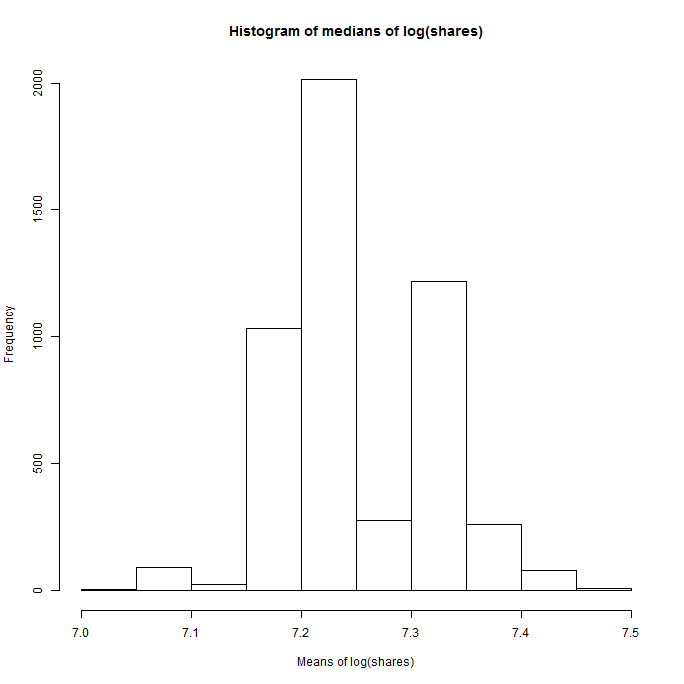
\includegraphics[width=0.95\linewidth]{hist_medians_of_log_shares.png} \\ a)}
\end{minipage}
\hfill
\begin{minipage}[h]{0.49\linewidth}
\center{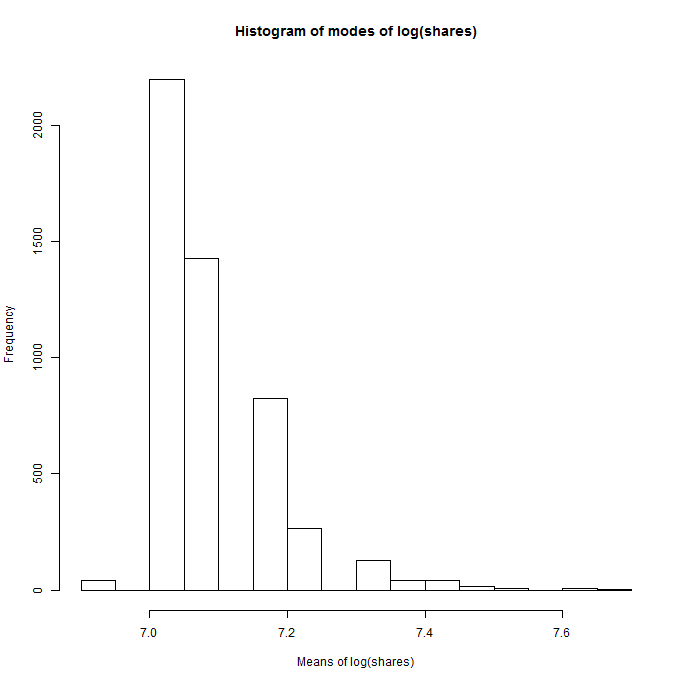
\includegraphics[width=0.95\linewidth]{hist_modes_of_log_shares.png} \\ b)}
\end{minipage}
\caption{Histograms of medians (a) and modes (b) of \texttt{$\log$(shares)}.}
\label{img:hist_medians_modes_log_shares}
\end{figure}

It is much more interesting to compute the confidence interval for median on initial scale, that is not  the median of logarithmic feature, but  the median of initial \texttt{shares} feature. Since the distribution of \texttt{shares} is more similar  to the power type distribution than to the normal one, it is better to choose the median as the central value due to the properties of median that were explained above.
In fact, we can use either pivotal or non-pivotal approaches to estimate a median because of the next theorem.

\begin{theorem}[Median Theorem, \cite{median_sample}]
Let a sample of size $n = 2m + 1$ with $n$ large be taken from an infinite population with a density
function $f(\bar{x})$ that is nonzero at the population median $\tilde{\mu}$ and continuously differentiable in a neighborhood of $\tilde{\mu}$. The sampling distribution of the median is approximately normal with mean $tilde{\mu}$ and variance $\frac{1}{8f(\tilde{\mu})^2 m}$.
\end{theorem}

The histogram of  sample medians  of \texttt{shares}  is presented at Figure \ref{img:hist_medians_modes_shares} (a), and computed confidence intervals are shown in the  Table  \ref{tbl:log_shares_and_shares_median_mode_CIs}. The mode's distribution is obviously far from normal (so we don't examine pivotal CI), and, as well as in the case of \texttt{$\log$(shares)} modes, the value of population mode is close to the left border of non-pivotal confidence interval. 

\begin{figure}[h]
\begin{minipage}[h]{0.49\linewidth}
\center{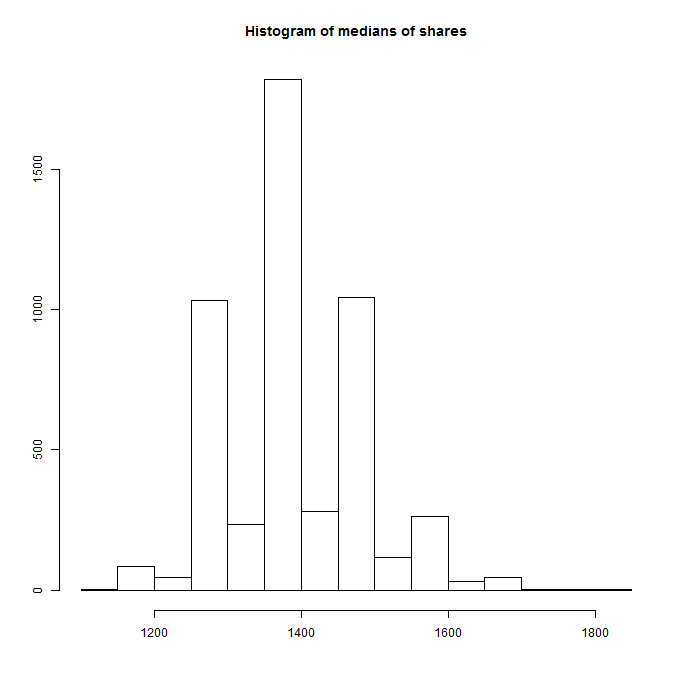
\includegraphics[width=0.95\linewidth]{hist_medians_of_shares.png} \\ a)}
\end{minipage}
\hfill
\begin{minipage}[h]{0.49\linewidth}
\center{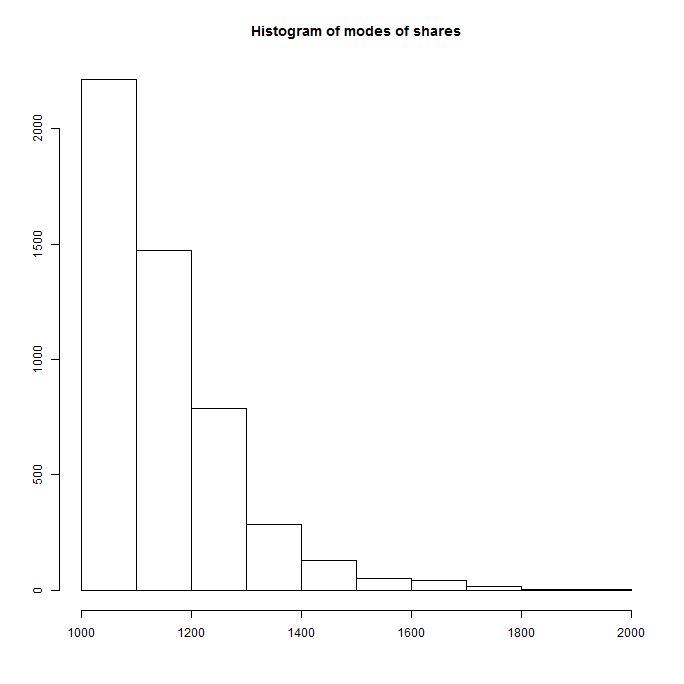
\includegraphics[width=0.95\linewidth]{hist_modes_of_shares.png} \\ b)}
\end{minipage}
\caption{Histograms of sample medians (a) and sample modes (b) of \texttt{shares}.}
\label{img:hist_medians_modes_shares}
\end{figure}

\begin{table}
\caption{95\% confidence intervals (CI's) for median and mode of \texttt{$\log$(shares)} and of \texttt{shares}} \label{tbl:log_shares_and_shares_median_mode_CIs}
\begin{center}
\begin{tabular}{|c|c|c||c|c|} 
 \hline
 & \multicolumn{2}{|c||}{\texttt{$\log$(shares)}} & \multicolumn{2}{|c|}{\texttt{shares}} \\ \hline 
& Median & Mode & Median & Mode  \\ \hline 
Value & 7.24 & 7.0 & 1400 & 1100 \\ \hline
Pivotal CI & (7.14; 7.36) & --- & (1257.76; 1571.5) & ---\\ \hline %(6.9; 7.26) (990.56; 1410.12) -- pivotals for modes
Nonpivotal CI & (7.17; 7.38) & (7.0; 7.3) & (1250; 1600) & (1100; 1500) \\ \hline
\end{tabular}
\end{center}
\end{table}  

\subsection*{Partitioning the population into two groups}
We split our \texttt{$\log$(shares)}  data according to the day, when the article was firstly published: workday or weekend. In our dataset we have seven dummy variables, indicating the day of publishing a news: \texttt{weekday\_is\_monday}, \texttt{weekday\_is\_tuesday}, \texttt{weekday\_is\_wed\-nes\-day}, \texttt{weekday\_is\_thursday}, \texttt{weekday\_is\_friday}, \texttt{weekday\_is\_saturday}, \texttt{weekday\_is\_sun\-day}. If we take entities, for which \texttt{weekday\_is\_saturday} or \texttt{weekday\_is\_sunday} are equal to 1, we will end up with the class \texttt{published\_on\_weekend}. All of the other entities will be considered as belonging to the class \texttt{published\_on\_workday}.  

Histograms of the sample means in each of the classes are shown in figure \ref{img:hist_log_shares_worday_weekend}. Each of the histrograms closely resembles the density of normal distribution, therefore pivotal and non-pivotal bootstrap methods should compute the similar confidence intervals (CI's). 95\% intervals for mean in each of the two groups are presented in Table \ref{tbl:workday_weekend_log_shares_CIs}.  

\begin{figure}[h!]
 \begin{center}
    \center 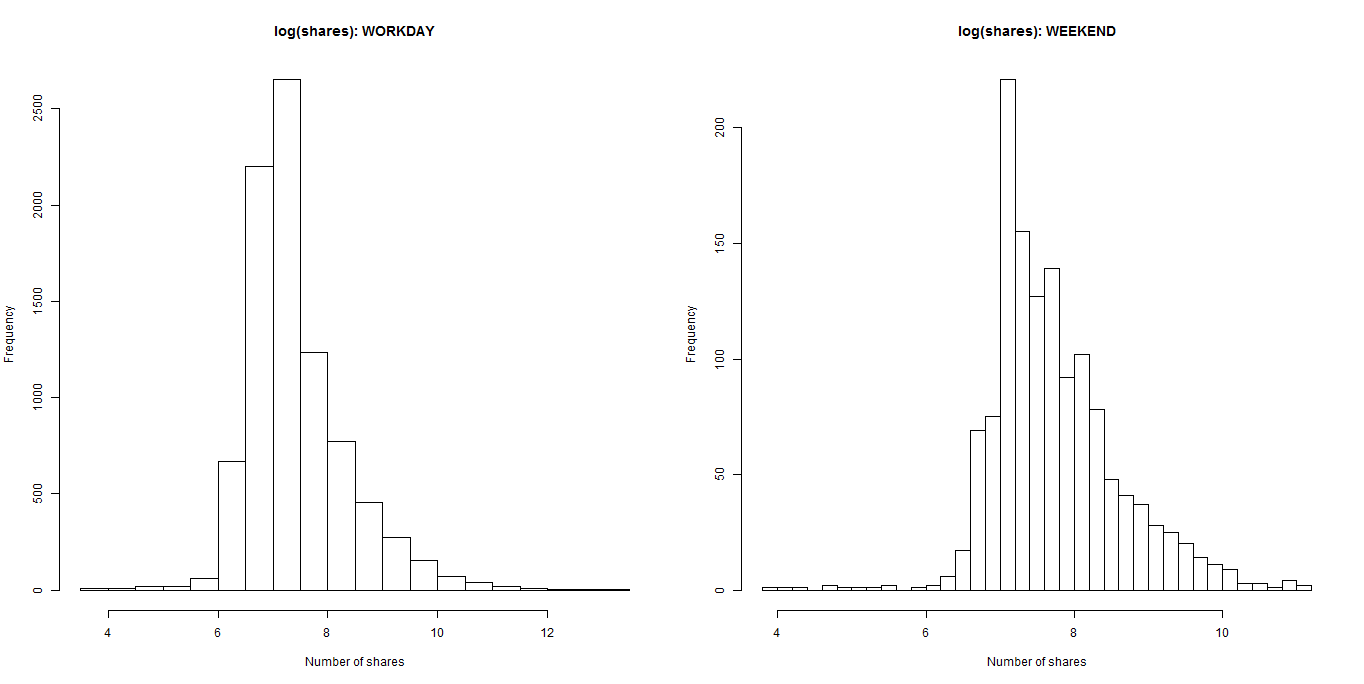
\includegraphics[width = 0.9\textwidth]{hist_log_shares_worday_weekend.png}
   \caption{30-bin histograms of \texttt{$\log$(shares)}, grouped by the day, when the article was published: workday (left) or weekend (right)}
   \label{img:hist_log_shares_worday_weekend}
 \end{center}
\end{figure} 

\begin{table}
\caption{Confidence intervals of mean of \texttt{$\log$(shares)} feature, grouped by a day, when the article was publishead: workday or weekend} \label{tbl:workday_weekend_log_shares_CIs}
\begin{center}
\begin{tabular}{|c|c|c|c|c|} 
 \hline
 & Workday & Weekend \\ \hline
Number of variables &  8660 & 1340 \\ \hline
Mean & 7.41 & 7.73 \\ \hline
Pivotal CI & (7.3; 7.5) & (7.63; 7.83)\\ \hline
Non-pivotal CI & (7.28; 7.54) & (7.6; 7.85)\\ \hline 
\end{tabular}
\end{center}
\end{table}

The CI of the mean in both classes do not intersect with each other, so we can claim with 95\% confidence that two means in these groups  are different.
 %But this is not a correct procedure, because ranges of means in workday and weekend articles groops intersected. 

\newpage
\section{Assignment 2. Linear regression.}

\subsection{Selection of features}

First of all, let's take a look at all continuous features' scatterplot to indentify which of them are linear dependent. 
Some features have nearly log-normal distributions, so, for more accurate and reliable linear regression we will logarithm these features.

\begin{figure}[h!]
 \begin{center}
    \center 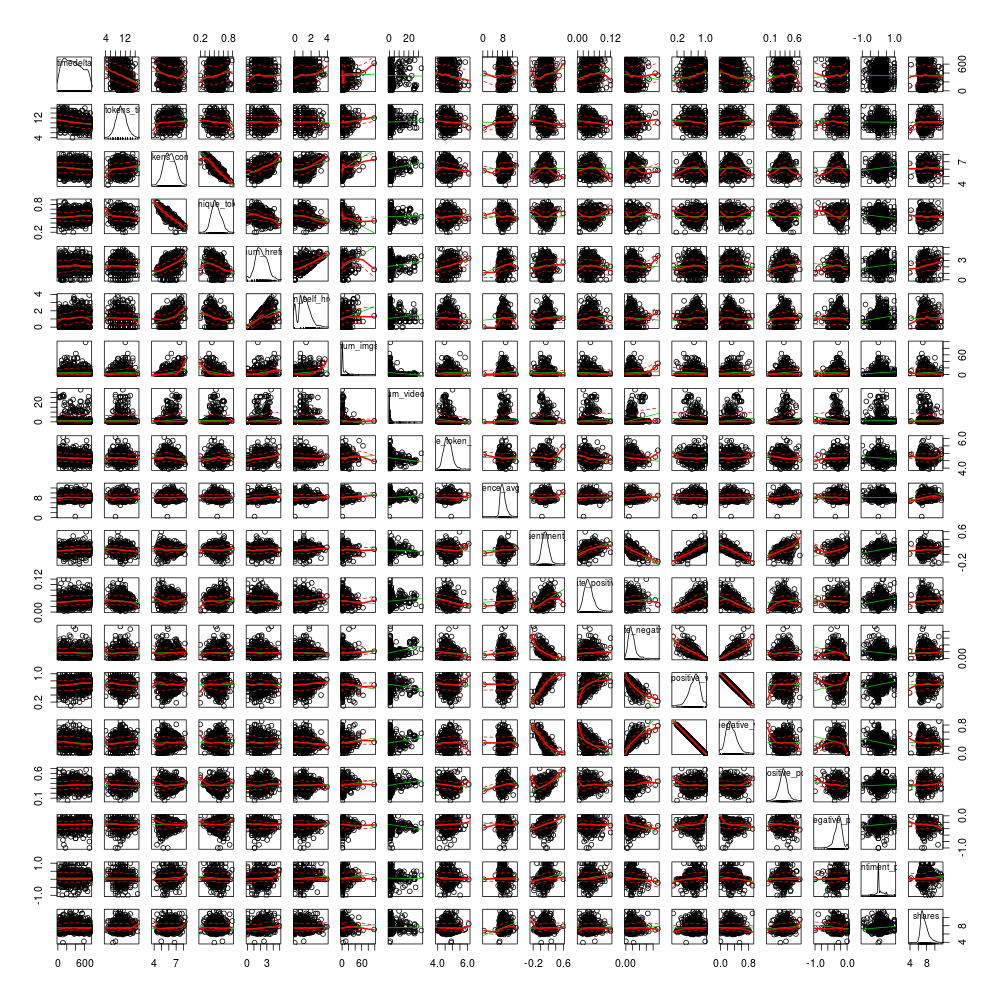
\includegraphics[width = 0.9\textwidth]{scatterplot_matrix_continuous_features_logged.png}
   \caption{Scatterplot matrix of all considered continuous features}
   \label{img:scatterplot_matrix_continuous_features_logged}
 \end{center}
\end{figure} 

As we can see from the scatterplot, the majority of pairs are not linear dependent. Fortunately, \texttt{global\_sentiment\_polarity} and \texttt{rate\_positive\_words} are linear dependent and we can easily understand why: they measure practicaly the same characteristic. The first feature is normalized from 0 to 1 (in out data from 0 to 0.7), the second one takes values from 0 to 1.

We will predict sentiment polarity over positive words rate. As we have rather heterogeneous data, let's make sure we won't be able to do our regression better with the help of groupping by \texttt{Channel} (Figure \ref{img:scatterplot_ratepositive_polarity}, a).

\begin{figure}[h]
\begin{minipage}[h]{0.49\linewidth}
\center{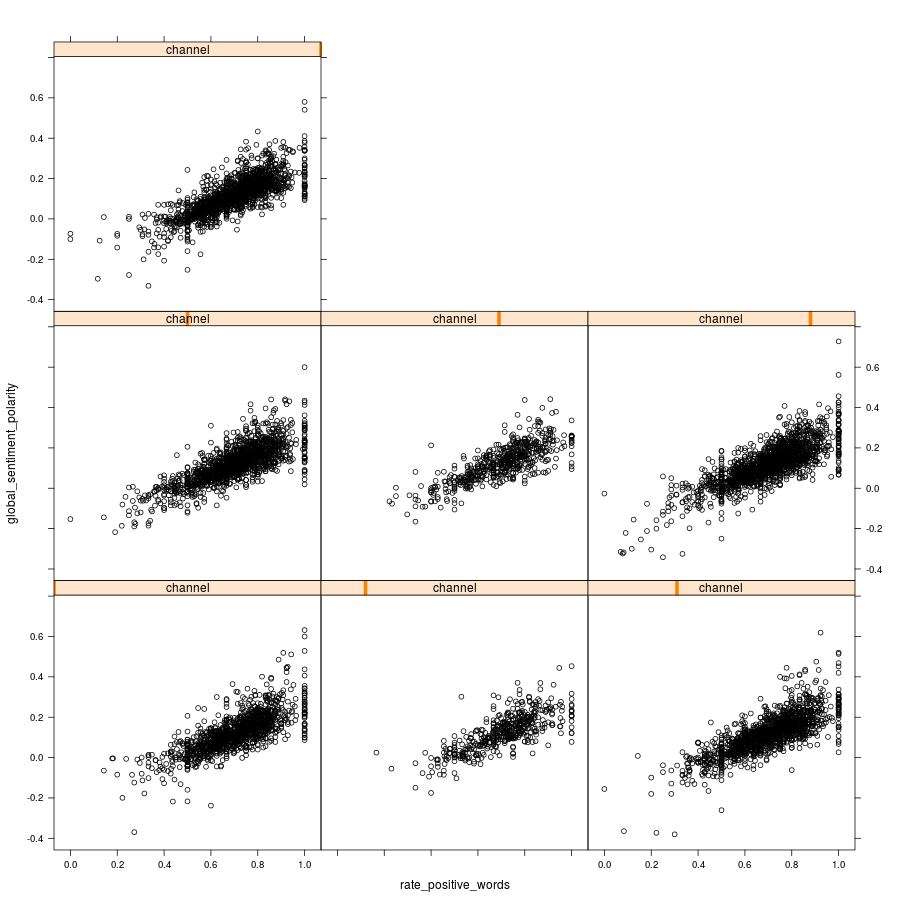
\includegraphics[width=0.95\linewidth]{scatterplot_ratepositive_polarity_groupped.png} \\ a)}
\end{minipage}
\hfill
\begin{minipage}[h]{0.49\linewidth}
\center{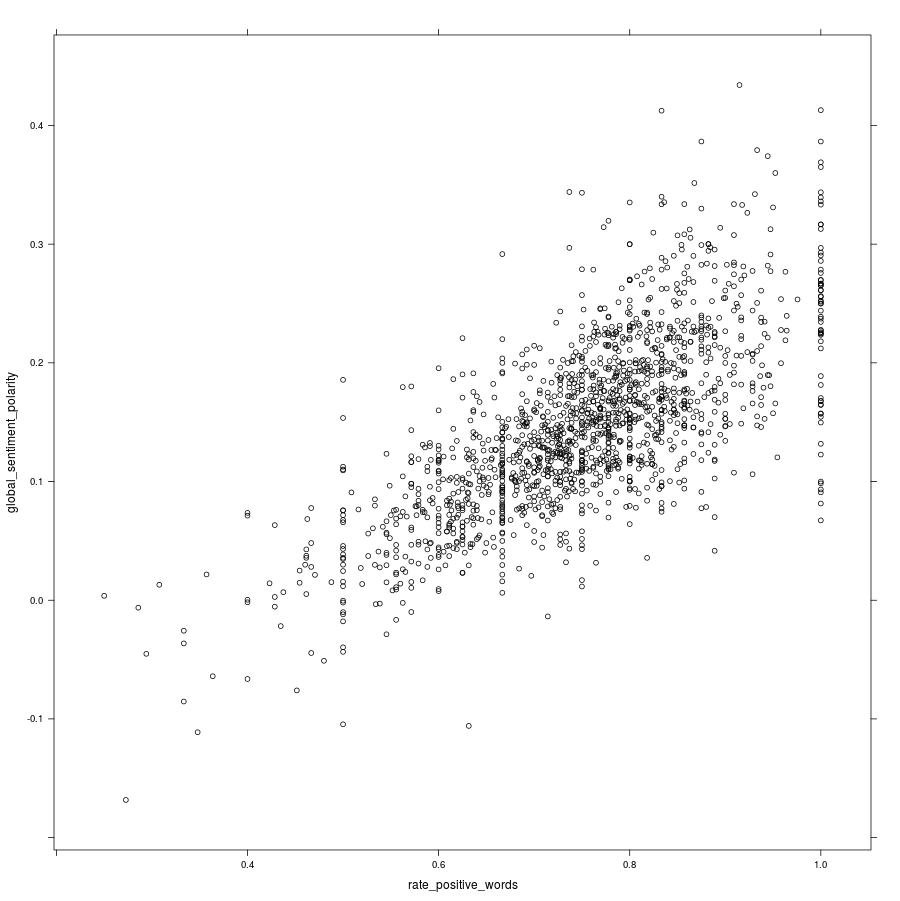
\includegraphics[width=0.95\linewidth]{scatterplot_ratepositive_polarity.png} \\ b)}
\end{minipage}
\caption{Groupped by channel (a) and only technical channel (b) dependece between \texttt{global\_sentiment\_polarity} and \texttt{rate\_positive\_words}.}
\label{img:scatterplot_ratepositive_polarity}
\end{figure}

All chanells looks very similar, and we dicided to consider only technical channel (just to reduce the sample size). After all these actions our scatterplot looks like at (Figure \ref{img:scatterplot_ratepositive_polarity}, b). Further at this section we will call the predicted and the prediction features just \texttt{global\_sentiment\_polarity} and \texttt{rate\_positive\_words}, implying we work with only one channel.
 
\subsection{Model of linear regression}

Using basic functions in R, we have built a linear regression with slope equals 0.4341 and intercept equals  -0.1788. The results of the regression you can see in Figure \ref{img:scatterplot_lr_ratepositive_polarity}.

\begin{figure}[h!]
 \begin{center}
    \center 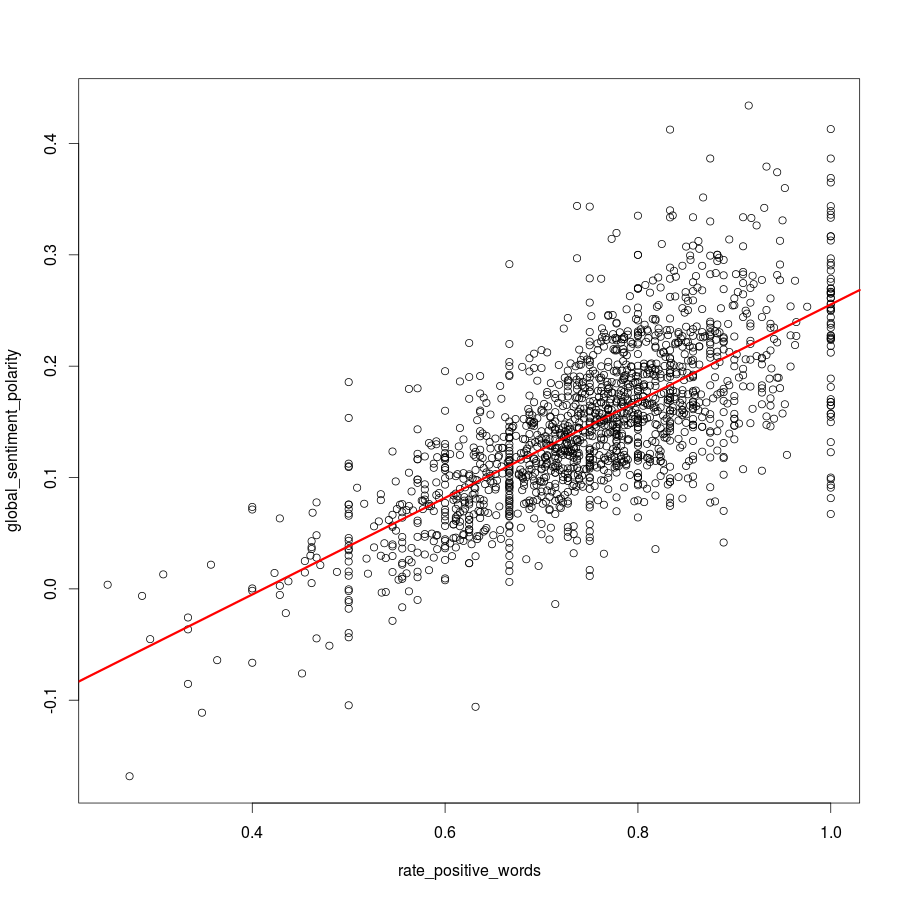
\includegraphics[width = 0.9\textwidth]{scatterplot_lr_ratepositive_polarity.png}
   \caption{}
   \label{img:scatterplot_lr_ratepositive_polarity}
 \end{center}
\end{figure} 

The slope is significantly positive (p-value equals 0) and it's not surpising: the more positive words are in the article, the more text is of positive polarity.

\subsection{Correlation and determinacy coefficients}

The correlation equals 0.7170736 and the coefficient of determination equals 0.5142 (ajusted is 0.5139). As we know from the definition of the coefficient of determination, $R^2$ measures of how well the regression line approximates the real data points and equals the ratio of explained variance. It's believed in practice that $R^2 > 0.5$ is acceptable, but not enough accurate. 

Particularly the value of 0.5139 means that about 51\% of variablility between the two   \texttt{global\_sentiment\_polarity} and \texttt{rate\_positive\_words} is captured by the linear model built with linear regression and the remaining 49\% of variability still remains unaccounted for. 

In another words the value of determination coefficient $R^2$ shows the rate of decrease of the variance of \texttt{global\_sentiment\_polarity} after its linear relation to \texttt{rate\_positive\_words} has been taken into account by the regression.

\subsection{Bootstrap}
We have conducted 5000 boostrap trials to estimate 95\%  confidence intervals of slope, intercept and correlation coefficient. 
The results are summarized by the histograms shown in the figures \ref{fig:bootsrap_intercept}-\ref{fig:bootsrap_correlation}. 

It can be easily seen that histograms are pretty similar to the normal type of distribution.  But let us prove that. 

We have  performed   the  Shapiro-Wilk normality test with intercept, slope and correlation coefficient bootstrap distributions. The results shown in the Table \ref{tbl:p_test_shapir_wilks}  are a little bit striking: with good p-value it is  trustworthy that intercept and slope boostrap samples are obtained from the normal distribution, but we could not say so about correlation coefficient samples data.

So for the correlation coefficient we compute CI using ranked quntiles.
The aforesaid results we  obtained are shown  in Table \ref{tbl:conf_intervals_intercept_slope_corr}.
It is worth to mention that the difference in estimating correlation coefficient CI using the assumption of normallity and without such is not very huge, but we think it is a good idea not only test normality of the data by it's visualization but also with statistical tests.

\begin{table}
	\centering
	\caption{Shapiro-Wilk normallity test p-value} \label{tbl:p_test_shapir_wilks} 
	\begin{tabular}{|c|c|}
		\hline  & 95\%  p-value \\ 
		\hline Intercept & 0.2279 \\ 
		\hline Slope  & 0.244  \\ 
		\hline Correlation &  5.621e-08 \\ 
		\hline 
	\end{tabular} 
\end{table} 




\begin{table}
\centering
	\caption{95\% confidence intervals (CI's) for intercept, slope, correlation coefficient based on bootrap techinque} \label{tbl:conf_intervals_intercept_slope_corr} 
\begin{tabular}{|c|c|}
	\hline  & 95\%  CI \\ 
	\hline Intercept &  (-0.209; -0.148) \\ 
	\hline Slope  & (0.392;  0.476)  \\ 
	\hline Correlation (normal) & (0.668; 0.765)   \\ 
	\hline Correlation (percentile) & (0.666,  0.763)   \\ 
	\hline 
\end{tabular} 
\end{table}
 
\begin{figure}[h!]
\centering
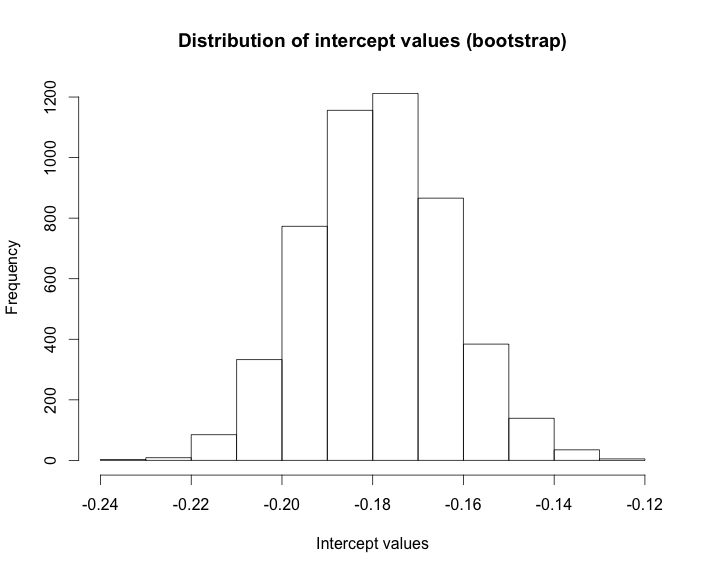
\includegraphics[width=0.7\linewidth]{images/bootsrap_intercept}
\caption{Distribution of intercept value of linear regression models built with each pair of sampled (\texttt{global\_sentiment\_polarity})  and  (\texttt{rate\_positive\_words}) using bootrsap}
\label{fig:bootsrap_intercept}
\end{figure}


\begin{figure}[h!]
\centering
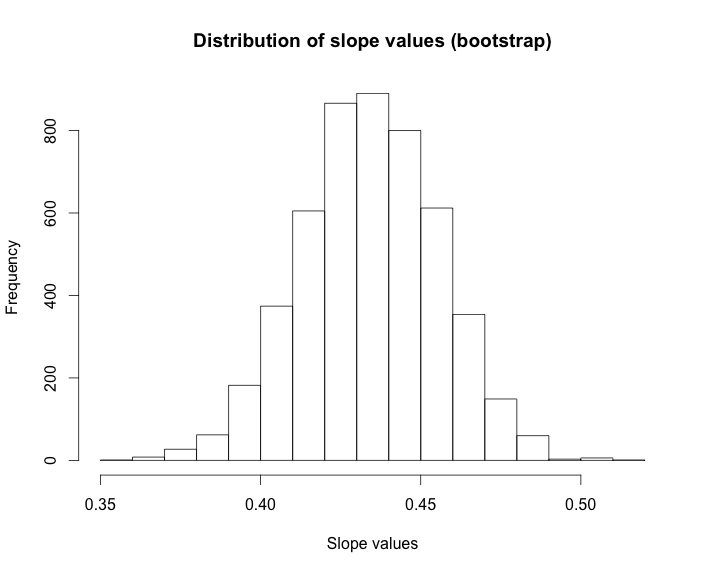
\includegraphics[width=0.7\linewidth]{images/bootsrap_slope}
\caption{Distribution of slope value of linear regression models built with each pair of sampled (\texttt{global\_sentiment\_polarity})  and  (\texttt{rate\_positive\_words}) using bootrsap}
\label{fig:bootsrap_slope}
\end{figure}



\begin{figure}[h!]
\centering
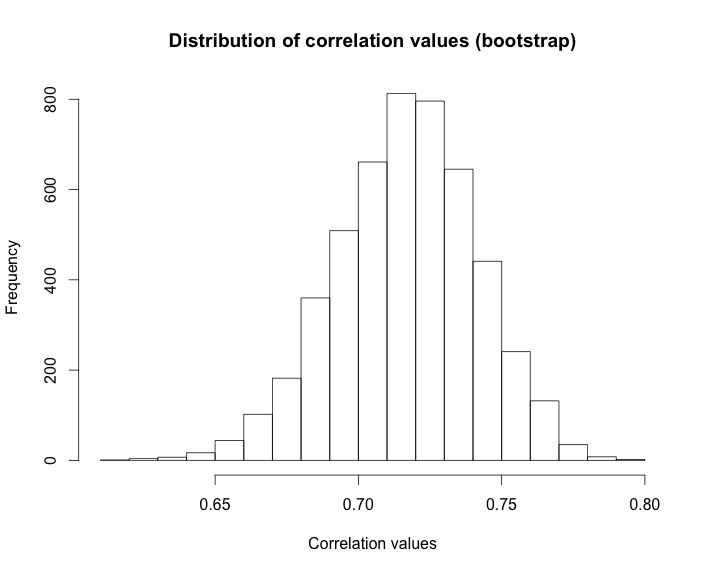
\includegraphics[width=0.7\linewidth]{images/bootsrap_correlation}
\caption{Distribution of correlation values between dependent variable (\texttt{global\_sentiment\_polarity}) and regressor (\texttt{rate\_positive\_words})}
\label{fig:bootsrap_correlation}
\end{figure}



\subsection{Average relative error}

Recall average relative error (ARE) and coefficient of determination (R$^2$) definitions:
\begin{gather*}
\text{ARE} = \frac{1}{N} \sum_{i=1}^{N}{\left\vert \frac{y_i - \hat{y}_i}{y_i} \right\vert}, \\
\text{R}^2 = 1 - \frac{\sum\limits_{i=1}^n (y_i - \hat{y}_i)^2}
                      {\sum\limits_{i=1}^n (y_i - \bar{y})^2}
\end{gather*}


\begin{lstlisting}[language=R]
mean( abs((y.feature - model$fitted.values)/y.feature) * 100) # in %
> 56.37 
summary_regression$r.squared * 100 # in %
> 51.419 
\end{lstlisting}

As we can see, considered values are reasonably close. But we should note that ARE is sensitive to the addition of a constant to all of the $y_i$ while R$^2$ is not. That is, we could obtain any arbitrary value of ARE keeping the coefficient of determination constant by adding some constants to $y_i$. 

It was suprise to us that ARE can be greater than 1 (which is the case if $y_i$ is much less than $y_i - \hat{y}_i$). 

According to all these facts one could conclude that comparing ARE and R$^2$  is meaningless without additional assumptions.


\subsection{Nature-inspired algorithm}
We will use nature-inspired algorithm to compute the parameters of linear regression that minimize the absolute relative error. If the target values of regression are $y_i$ and predicted by linear regression values are $\hat{y}_i$, the  absolute relative error is:
\begin{equation}
\frac{1}{N} \sum_{i=1}^{N}{\left\vert \frac{y_i - \hat{y}_i}{y_i} \right\vert}.
\end{equation}

We have implemented algorithm similar to the one, which is described in \cite{CCODA_Mirkin}, but we will minimize the function \texttt{delta(coefficients, x, y)}, which looks like
\begin{lstlisting}[language=R]
delta <- function(coefficients, x,y){
  a = coefficients[1]; b = coefficients[2]
  yp <- a*x + b
  esq <- mean( abs((y - yp)/y) ) 
} 
\end{lstlisting}

We also need the function that compute permissible limits for coefficients. Let look at two values of target $y_i = a \cdot x_i + b$ and $y_j = a \cdot x_j + b$ ($i \neq j$) and express $a$, $b$ in terms of $x$ and $y$:
\begin{equation*}
a_{ij} = \frac{y_j - y_i}{x_j - x_i}, \ b_{ij} = \frac{y_i x_j - y_j x_i}{x_j - x_i}.
\end{equation*}
And then we calculate $\max$ and $\min$ of coefficients $a$ and $b$ among all pairs $(x_i,y_i)$ and $(x_j,y_j)$. 

%That implemented in the function \texttt{ddr(x, y)}.  The code of this function and function \texttt{nlr(x,y, popSize = 15, iter = 5000)} is given below.

Using the nature-inspired approach (we have implemented it in R-function nlr) we obtained the following values
of slope ($a$) and intercept ($b$) and value of relative error:
\begin{lstlisting}[language=R]
# The regression model: y.feature = a * x.feature + b
# Coefficients of slope and intercept respectively:
model.nlr <- nlr(x.feature, y.feature) 
> 0.3514270 -0.1421007

# Value of relative error:
eps.nlr <- y.feature - model.nlr[1]*x.feature - model.nlr[2]
mean( abs(eps.nlr / y.feature) ) * 100
> 50.54
\end{lstlisting}

Comparing the values of two relative errors, we can see that nature-inspired approach reduce its value by a few percent. 
%
%The main code of nature-inspired approach:
%\begin{lstlisting}[language=R]
%# ddr determine the permissible limits for slope and intercept 
%ddr <- function(x,y){
%  ll <- length(x)
%  eps <- 0.05
%  a <- ldply(1:(ll-1), function(i){
%    v <- sapply((i+1):ll, function(j) 
%      ifelse(abs(x[i] - x[j]) > eps, 
%        (y[i] - y[j])/(x[i] - x[j]), NA))
%    c(min(v, na.rm = TRUE), max(v, na.rm = TRUE))
%  })
%  b <- ldply(1:(ll-1), function(i){
%    v <- sapply((i+1):ll, function(j) 
%      ifelse(abs(x[i] - x[j]) > eps, 
%        (y[j]*x[i] - y[i]*x[j])/(x[i] - x[j]), NA))
%    c(min(v, na.rm = TRUE), max(v, na.rm = TRUE))
%  })
%  
%  list(a.boundaries = c(min(a[,1]), max(a[,2])), 
%       b.boundaries = c(min(b[,1]), max(b[,2])))
%}
%
%# Realization of nature-inspired approach
%# The code is similar to the Matlab code from CCODA textbook 
%nlr <- function(x,y, popSize = 15, iter = 5000){
%  ll <- length(x)
%  bounds <- ddr(x,y) #intervals for coefficients
%  lb <- c(bounds[[1]][1],bounds[[2]][1])
%  rb <- c(bounds[[1]][2],bounds[[2]][2])
%  feas <- matrix(c(rep(rb[1]-lb[1],popSize),rep(rb[2]-lb[2],popSize)),
%   ncol=2) * cbind(rnorm(popSize),rnorm(popSize)) +
%       matrix(c(rep(lb[1],popSize), rep(lb[2],popSize)), ncol = 2)
%  flag = 1; count = 0; funp = 0
%  vv <- apply(feas, 1, function(d) delta(d, x, y))  
%  funi <- min(vv); ini <- which.min(vv); soli <- feas[ini,]
%  si = 1
%  while (flag == 1){
%    count <- count + 1
%    feas <- feas + cbind(rnorm(popSize),rnorm(popSize))
%    feas <- t(apply(feas, 1, function(x) ifelse(x > lb, 
%              ifelse(x < rb, x, rb), lb)))
%    vec <- apply(feas, 1, function(d) delta(d, x, y)) 
%    fun <- min(vec); un <- which.min(vec); sol <- feas[un,]
%    wf <- max(vec); wi <- which.max(vec); wun <-feas[wi,]
%    if (wf > funi){
%      feas[wi,] <- soli 
%      vec[wi] <- funi
%    } 
%    if (fun < funi) {
%      soli <- sol; funi <- fun
%    }
%    if (count >= iter) { flag = 0 }
%    residvar <- funi/var(y)
%  }
%  a <- soli[1]; b <- soli[2]
%  c(a,b)
%}
%\end{lstlisting}

In R-language there is a package \texttt{genalg} with function \texttt{rbga} that implement this approach. The results obtained with function \texttt{rbga} are very close to the results described above:
\begin{lstlisting}[language=R]
# The regression model: y.feature = a * x.feature + b
# Calculate the permissible limits for a and b 
bound <- ddr(x.feature, y.feature)
bounds.min <- c(bound[[1]][1],bound[[2]][1]) # (a.min, b.min) 
bounds.max <- c(bound[[1]][2],bound[[2]][2]) # (a.max, b.max)

rbga.res <- rbga(bounds.min, bounds.max, popSize = 30, iters = 5000,
   evalFunc = function(coefs) delta(coefs, x.feature, y.feature))

# Results (we need to take a look at "Best Solution")
summary(rbga.res)
> GA Settings
  Type  = floats chromosome
  Population size       = 30
  Number of Generations = 5000
  Elitism               = 6
  Mutation Chance       = 0.333333333333333
  
  Search Domain
  Var 1 = [-6.674999999946,6.47188552188199]
  Var 2 = [-5.27885519411197,5.97499999995278]
  
  GA Results
  Best Solution : 0.347731933975272 -0.146302152742407 

# Value of relative error:
delta(c(0.3477, -0.1463), x.feature, y.feature)) * 100
> 49.93
\end{lstlisting}

\clearpage
\documentclass{article}\usepackage[]{graphicx}\usepackage[]{color}
%% maxwidth is the original width if it is less than linewidth
%% otherwise use linewidth (to make sure the graphics do not exceed the margin)
\makeatletter
\def\maxwidth{ %
  \ifdim\Gin@nat@width>\linewidth
    \linewidth
  \else
    \Gin@nat@width
  \fi
}
\makeatother

\definecolor{fgcolor}{rgb}{0.345, 0.345, 0.345}
\newcommand{\hlnum}[1]{\textcolor[rgb]{0.686,0.059,0.569}{#1}}%
\newcommand{\hlstr}[1]{\textcolor[rgb]{0.192,0.494,0.8}{#1}}%
\newcommand{\hlcom}[1]{\textcolor[rgb]{0.678,0.584,0.686}{\textsf{#1}}}%
\newcommand{\hlopt}[1]{\textcolor[rgb]{0,0,0}{#1}}%
\newcommand{\hlstd}[1]{\textcolor[rgb]{0.345,0.345,0.345}{#1}}%
\newcommand{\hlkwa}[1]{\textcolor[rgb]{0.161,0.373,0.58}{\textbf{#1}}}%
\newcommand{\hlkwb}[1]{\textcolor[rgb]{0.69,0.353,0.396}{#1}}%
\newcommand{\hlkwc}[1]{\textcolor[rgb]{0.333,0.667,0.333}{#1}}%
\newcommand{\hlkwd}[1]{\textcolor[rgb]{0.737,0.353,0.396}{\textbf{#1}}}%

\usepackage{framed}
\makeatletter
\newenvironment{kframe}{%
 \def\at@end@of@kframe{}%
 \ifinner\ifhmode%
  \def\at@end@of@kframe{\end{minipage}}%
  \begin{minipage}{\columnwidth}%
 \fi\fi%
 \def\FrameCommand##1{\hskip\@totalleftmargin \hskip-\fboxsep
 \colorbox{shadecolor}{##1}\hskip-\fboxsep
     % There is no \\@totalrightmargin, so:
     \hskip-\linewidth \hskip-\@totalleftmargin \hskip\columnwidth}%
 \MakeFramed {\advance\hsize-\width
   \@totalleftmargin\z@ \linewidth\hsize
   \@setminipage}}%
 {\par\unskip\endMakeFramed%
 \at@end@of@kframe}
\makeatother

\definecolor{shadecolor}{rgb}{.97, .97, .97}
\definecolor{messagecolor}{rgb}{0, 0, 0}
\definecolor{warningcolor}{rgb}{1, 0, 1}
\definecolor{errorcolor}{rgb}{1, 0, 0}
\newenvironment{knitrout}{}{} % an empty environment to be redefined in TeX

\usepackage{alltt}

\usepackage[utf8]{inputenc}
%\usepackage[cp1251]{inputenc}
\usepackage[english]{babel}
\usepackage{indent first}
\usepackage[top=2 cm, bottom = 2 cm, left = 3 cm, right = 1.5 cm]{geometry}
\usepackage{amsmath}
\usepackage{amssymb}
\usepackage{amsthm}
\usepackage{graphicx}
\usepackage{wrapfig}
\usepackage{listings}
\usepackage{ mathrsfs }
\usepackage{subcaption}
\graphicspath{{images/}}
\renewcommand{\baselinestretch}{1.1}

\newtheorem*{theorem}{Theorem}
\IfFileExists{upquote.sty}{\usepackage{upquote}}{}
\begin{document}
%<*includetag>
\section{Assignment 4}
\subsection{Selection and building nominal features}
In our dataset we have several binary features, such as weekdays (\texttt{weekday\_is\_monday}, \texttt{weekday\_is\_tuesday} and so on) and belonging to one of the channels (\texttt{data\_channel\_is\_lifestyle}, \texttt{data\_channel\_is\_entertainment} and so on). Therefore we built two nominal features:
\begin{itemize}
\item channel: integer values ranging between 1 and 6 ('Lifestyle', 'Entertainment', 'Business', 'Social Media', 'Tech', 'World')
\item weekday: integer values ranging between 1 and 7 
\end{itemize}

To obtain the third nominal feature we divide into four parts the feature \texttt{timedelta}: days between the article publication and the dataset acquisition.
\begin{knitrout}
\definecolor{shadecolor}{rgb}{0.969, 0.969, 0.969}\color{fgcolor}\begin{kframe}
\begin{alltt}  
\hlstd{timegroup} \hlkwb{<-} \hlkwa{cut}\hlstd{(data$timedelta, breaks = 4})
\end{alltt}
\end{kframe}
\end{knitrout} 

And we break range of values of \texttt{timedelta} into intervals: $(7.28,189]$, $(189,370]$, $(370,550]$, $(550,732]$

\subsection{Contingency tables over features}
Conditional frequency tables over introdused nominal fetures are obtained with R-function \texttt{table} as showned below and results are presented at Tables \ref{tbl:cont_table_ch_timed} -- \ref{tbl:cont_table_timed_week}.
\begin{knitrout}
\definecolor{shadecolor}{rgb}{0.969, 0.969, 0.969}\color{fgcolor}\begin{kframe}
\begin{alltt}  
table(data$channel, data$timegroup)
table(data$channel, data$weekday)
\end{alltt}
\end{kframe}
\end{knitrout} 

\begin{table}[h]
\begin{center}
\small
\begin{minipage}[h]{0.45\linewidth}
\caption{Conditional frequency table over \texttt{channel} and \texttt{timegroup}} \label{tbl:cont_table_ch_timed}
\begin{tabular}{|c|c|c|c|c|} 
 \hline
  &(7.28,189] &(189,370]& (370,550] &(550,732] \\ \hline
  0  &      412   &    327   &    361   &    381 \\ \hline
  1  &      120   &     93   &    130   &    183 \\ \hline
  2  &      573   &    473   &    341   &    348 \\ \hline
  3  &      392   &    408   &    410   &    446 \\ \hline
  4  &       81   &    154   &    163   &    192 \\ \hline
  5  &      401   &    469   &    491   &    492 \\ \hline
  6  &      901   &    564   &    373   &    321 \\ \hline
\end{tabular}
\end{minipage}
\hfill 
\begin{minipage}[h]{0.45\linewidth}
\caption{Conditional frequency table over \texttt{channel} and \texttt{weekday}} \label{tbl:cont_table_ch_week}
\begin{tabular}{|c|c|c|c|c|c|c|c|} 
 \hline
     &1 & 2 & 3 & 4 & 5 & 6 & 7 \\ \hline
  0  & 224 & 256 &253 &257 &238 &112 &141 \\ \hline
  1  & 80 & 95 &  92 & 85  &69  &46  &59 \\ \hline
  2  & 317 & 332 & 311 & 287 & 241 & 95 & 152 \\ \hline
  3  & 277 & 293 & 371 & 319 & 245 & 57 & 94 \\ \hline
  4  & 88 & 116 &105& 115 & 88 & 44 & 34 \\ \hline
  5  & 316 & 372 & 358 & 344 & 244 & 125 & 94\\ \hline
  6  & 360& 379& 399& 392& 342& 136& 151 \\ \hline
\end{tabular}
\end{minipage}
\end{center}
\end{table}

Quetelet relative index tables over our nominal fetures we obtain with the function:
\begin{knitrout}
\definecolor{shadecolor}{rgb}{0.969, 0.969, 0.969}\color{fgcolor}\begin{kframe}
\begin{alltt}  
getQueteletIndex \hlkwb{<-} \hlkwa{function}(v1, v2) {
  size \hlkwb{<-} length(v1)
  cont.table  \hlkwb{<-} table(v1, v2)
  row.sums  \hlkwb{<-} rowSums(cont.table)
  col.sums  \hlkwb{<-} colSums(cont.table)
  norm.cont.table  \hlkwb{<-}  cont.table / size
  norm.row.sums  \hlkwb{<-} row.sums / size
  norm.col.sums  \hlkwb{<-} col.sums / size
  list(Quetelet = norm.cont.table / (norm.row.sums %*% t(norm.col.sums)) - 1,
       PearsonIndexMatrix = (-norm.row.sums %*% t(norm.col.sums) + norm.cont.table) /
          sqrt(norm.row.sums %*% t(norm.col.sums)))
}
\end{alltt}
\end{kframe}
\end{knitrout}

The results (in percent) are  presented at Tables \ref{tbl:quet_table_ch_timed}, \ref{tbl:quet_table_ch_week}. 
\begin{table}[h]
\footnotesize
\begin{center}
\begin{minipage}[h]{0.4\linewidth}
\caption{Quetelet relative index table over \texttt{channel} and \texttt{timegroup}} \label{tbl:quet_table_ch_timed}
\begin{tabular}{|c|c|c|c|c|} 
 \hline
  &(7.28,189] &(189,370]& (370,550] &(550,732] \\ \hline
  0&      -3.41  &  -11.26&      7.43&      8.87 \\ \hline
  1 &    -20.79  &  -28.94&      8.92&\textbf{47.23} \\ \hline
  2  &14.67 &\textbf{9.57}&    -13.38&    -15.12 \\ \hline
  3&     -17.81 &    -0.97&      9.12&     13.98 \\ \hline
  4 &    -52.33 & 4.91&\textbf{21.76}&     37.72 \\ \hline
  5  &   -24.86&      1.73&     16.78&     12.36 \\ \hline
  6&\textbf{44.90}&   5.00&    -23.86&    -37.08 \\ \hline
\end{tabular}
\end{minipage}
\hfill 
\begin{minipage}[h]{0.5\linewidth}
\caption{Quetelet relative index table over \texttt{channel} and \texttt{weekday}} \label{tbl:quet_table_ch_week}
\begin{tabular}{|c|c|c|c|c|c|c|c|} 
 \hline
     &1 & 2 & 3 & 4 & 5 & 6 & 7 \\ \hline
  0  &-9.00&  -6.21&  -9.57&  -3.54 &  9.54&  22.97&  31.32 \\ \hline
  1 & -8.49&  -2.00&  -7.41& -10.17 &-10.58&\textbf{42.20}&\textbf{54.71}\\ \hline
  2&\textbf{9.93}&   3.83&  -5.11&  -8.05 & -5.31& -10.97&  20.84 \\ \hline
  3&   0.64&  -4.00&\textbf{18.60}&   7.08 &  0.85& -44.03& -21.71 \\ \hline
  4& -10.26&   6.68&  -5.79&\textbf{8.35}&  1.67&  21.26& -20.51 \\ \hline
  5&   2.61&\textbf{8.93}&   2.28&   3.19 &-10.24&   9.69& -30.03 \\ \hline
  6&   0.33&  -4.75&  -2.17&   0.93 &\textbf{7.98}&   2.43&  -3.53 \\ \hline
\end{tabular}
\end{minipage}
\end{center}
\end{table}

As we can see from the Table \ref{tbl:quet_table_ch_timed}, \texttt{timegroup} is dependent with \texttt{channel} in some values. For example, we observe rather big Quetelet relative index between \textsf{Entartanment channel} and \textsf{4th time-group}. \footnote{WHY????}
In addition, we can't reject a dependence between \textsf{World channel} and \textsf{1st time-group}. It can be caused by not random sampling or by some extra-ordinary events with great response in the world.

Table \ref{tbl:quet_table_ch_week} provides us less surprising and more predictable results: all channels are almost independent with weekdays inspite of \textsf{Entartanment channel} and \textsf{Weekend}. This result is easy to understand: users visit Mashable at weekends to amuse themselves. \footnote{To fix.}


\subsection{$\chi^2$--summary Quetelet index}


\begin{table}[ht]
\centering
\begin{tabular}{|c|c|c|c|c|c|}
  \hline
 &(7.28,189] & (189,370] & (370,550] & (550,732] & Sum \\ 
  \hline
0 & -0.007 (0.00005) & -0.02161 (0.0004) & 0.01362 (0.0002) & 0.01659 (0.0003) & (0.00098) \\  \hline
1 & -0.02558 (0.0006) & -0.03310 (0.001) & 0.00975 (0.0001) & 0.05266 (0.003)  & (0.0046)  \\ \hline
2 & 0.03280 (0.001) & 0.01989 (0.0004) & -0.02655 (0.0007) & -0.03061 (0.0009) & (0.003)   \\ \hline
3 & -0.03889 (0.0015) & -0.00198 (0) & 0.01767 (0.0003) & 0.02765 (0.0008)     & (0.0026)  \\ \hline
4 & -0.06821 (0.0047) & 0.00595  (0.00004) & 0.02518 (0.0006) & 0.04453 (0.002)& (0.0073) \\ \hline
5 & -0.05743 (0.0033) & 0.00371 (0.00001) & 0.03441 (0.0012) & 0.02587 (0.0006)& (0.005)  \\ \hline
6 & 0.11197 (0.013) & 0.01158 (0.00013) & -0.05281 (0.00279) & -0.08375 (0.007)& (0.0225)  \\ \hline
Sum & (0.0237)      & (0.002)			& (0.006)			 & (0.0144)		   & (0.04624) \\ \hline
\end{tabular}
\caption{$\chi^2$--summary Quetelet index over \texttt{channel} and \texttt{timegroup}} \label{tbl:quet_table_ch_week}
\end{table}

\begin{table}[ht]
\centering
\footnotesize
\begin{tabular}{|c|c|c|c|c|c|c|c|c|}
  \hline
 & 1 & 2 & 3 & 4 & 5 & 6 & 7 & Sum \\ 
  \hline
0 & -0.014  (0) & -0.01  (0) & -0.016  (0) & -0.006  (0) & 0.014  (0) & 0.022  (0) & 0.032  (0.001) & (0.002) \\  \hline
1 & -0.008  (0) & -0.002  (0) & -0.007  (0) & -0.01  (0) & -0.009  (0) & 0.024  (0.001) & 0.034  (0.001) & (0.002) \\  \hline
2 & 0.017  (0) & 0.007  (0) & -0.009  (0) & -0.014  (0) & -0.008  (0) & -0.011  (0) & 0.023  (0.001) & (0.001) \\  \hline
3 & 0.001  (0) & -0.007  (0) & 0.033  (0.001) & 0.012  (0) & 0.001  (0) & -0.044  (0.002) & -0.024  (0.001) & (0.004) \\  \hline
4 & -0.01  (0) & 0.007  (0) & -0.006  (0) & 0.009  (0) & 0.002  (0) & 0.013  (0) & -0.013  (0) & (0.001) \\  \hline
5 & 0.005  (0) & 0.017  (0) & 0.004  (0) & 0.006  (0) & -0.017  (0) & 0.01  (0) & -0.035  (0.001) & (0.002) \\  \hline
6 & 0.001  (0) & -0.009  (0) & -0.004  (0) & 0.002  (0) & 0.014  (0) & 0.003  (0) & -0.004  (0) & (0) \\  \hline
Sum & (0.001) & (0.001) & (0.002) & (0.001) & (0.001) & (0.003) & (0.005) &  (0.0124)\\ 
   \hline
\end{tabular}
\caption{$\chi^2$--summary Quetelet index over \texttt{channel} and \texttt{weekday}} \label{tbl:quet_table_ch_week}
\end{table}

%</includetag>
\end{document}


\bibliographystyle{ugost2008ls}
\bibliography{references.bib}

\end{document}
